\documentclass{article}

\usepackage[utf8]{inputenc}
\usepackage[bottom=2cm, top=2cm, left=2cm, right=2cm]{geometry}
\usepackage{verbatim}
\usepackage{tikz}
\usetikzlibrary{shapes}

\title{Lista - Árvores B}
\author{Vinícius Couto Tasso}
\date{}

\begin{document}

\maketitle
         
\begin{enumerate}

\item \textbf{Considerando a árvore a seguir (o grau mínimo para essa árvore B é $t=3$), realize, nessa ordem, as seguintes operações: \texttt{RM(S); ADD(D); RM(E); ADD(M); RM(L); RM(X); ADD(F); RM(N); RM(J)}. Para cada remoção, identifique o caso no qual se enquadra.}

\input{tree.tex}

\texttt{RM(S)} $\rightarrow$ Caso 1

\input{rm-s.tex}

\texttt{RM(E)} $\rightarrow$ Caso 2A

\begin{center}
    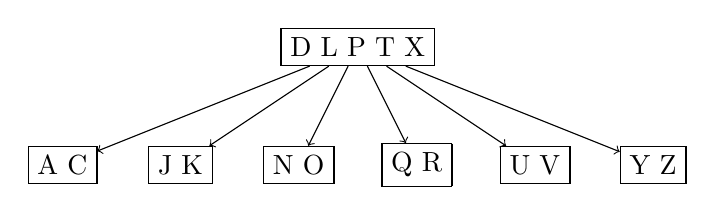
\begin{tikzpicture}
    \tikzstyle{btree}=[rectangle split, rectangle split horizontal, rectangle split ignore empty parts, draw]
    \tikzstyle{every node}=[btree]
    \tikzstyle{level 1}=[sibling distance=15mm]
   
    \node {D L P T X} [->]
        child {node {A C}}   
        child {node {J K}}
        child {node {N O}}
        child {node {Q R}}
        child {node {U V}}
        child {node {Y Z}
        };
    
    \end{tikzpicture}
\end{center}

\texttt{RM(L)} $\rightarrow$ Caso 2B

\input{rm-l.tex}

\texttt{RM(X)} $\rightarrow$ Caso 2C

\begin{center}
    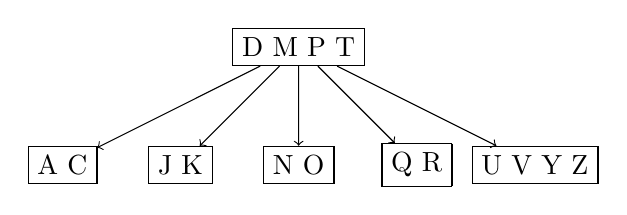
\begin{tikzpicture}
    \tikzstyle{btree}=[rectangle split, rectangle split horizontal, rectangle split ignore empty parts, draw]
    \tikzstyle{every node}=[btree]
    \tikzstyle{level 1}=[sibling distance=15mm]
   
    \node {D M P T} [->]
        child {node {A C}}   
        child {node {J K}}
        child {node {N O}}
        child {node {Q R}}
        child {node {U V Y Z}
        };
    
    \end{tikzpicture}
\end{center}

\newpage

\texttt{RM(N)} $\rightarrow$ Caso 3A

\begin{center}
    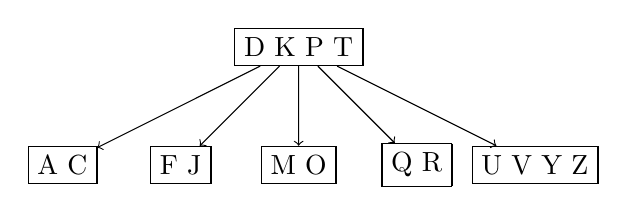
\begin{tikzpicture}
    \tikzstyle{btree}=[rectangle split, rectangle split horizontal, rectangle split ignore empty parts, draw]
    \tikzstyle{every node}=[btree]
    \tikzstyle{level 1}=[sibling distance=15mm]
   
    \node {D K P T} [->]
        child {node {A C}}   
        child {node {F J}}
        child {node {M O}}
        child {node {Q R}}
        child {node {U V Y Z}
        };
    
    \end{tikzpicture}
\end{center}

\texttt{RM(J)} $\rightarrow$ Caso 3B

\begin{center}
    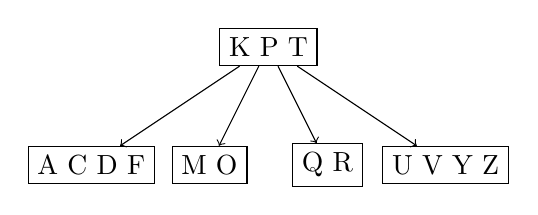
\begin{tikzpicture}
    \tikzstyle{btree}=[rectangle split, rectangle split horizontal, rectangle split ignore empty parts, draw]
    \tikzstyle{every node}=[btree]
    \tikzstyle{level 1}=[sibling distance=15mm]
   
    \node {K P T} [->]
        child {node {A C D F}}
        child {node {M O}}
        child {node {Q R}}
        child {node {U V Y Z}
        };
    
    \end{tikzpicture}
\end{center}

\end{enumerate}

\end{document}
